%\chapter{Vorlesung}
%\subsection[Laufzeit für Dinic-Algo. bei Flussnetzwerken mit Einheitskapazität]{Laufzeit für Dinic-Algorithmus bei Flussnetzwerken mit Einheitskapazität}
%\[ \mathcal{O}\left( \min\left\{ |E|^\frac{1}{2},|V|^\frac{2}{3} \right\}\cdot|E| \right) \]
\paragraph{2. Fall}
\subparagraph{1. Phase} Führe $2\cdot |V|^\frac{2}{3}$ Sperrflussberechnungen durch.
$\Rightarrow~\delta_f(s,t)>2\cdot|V|^\frac{2}{3}$
\begin{figure}[h]
\centering
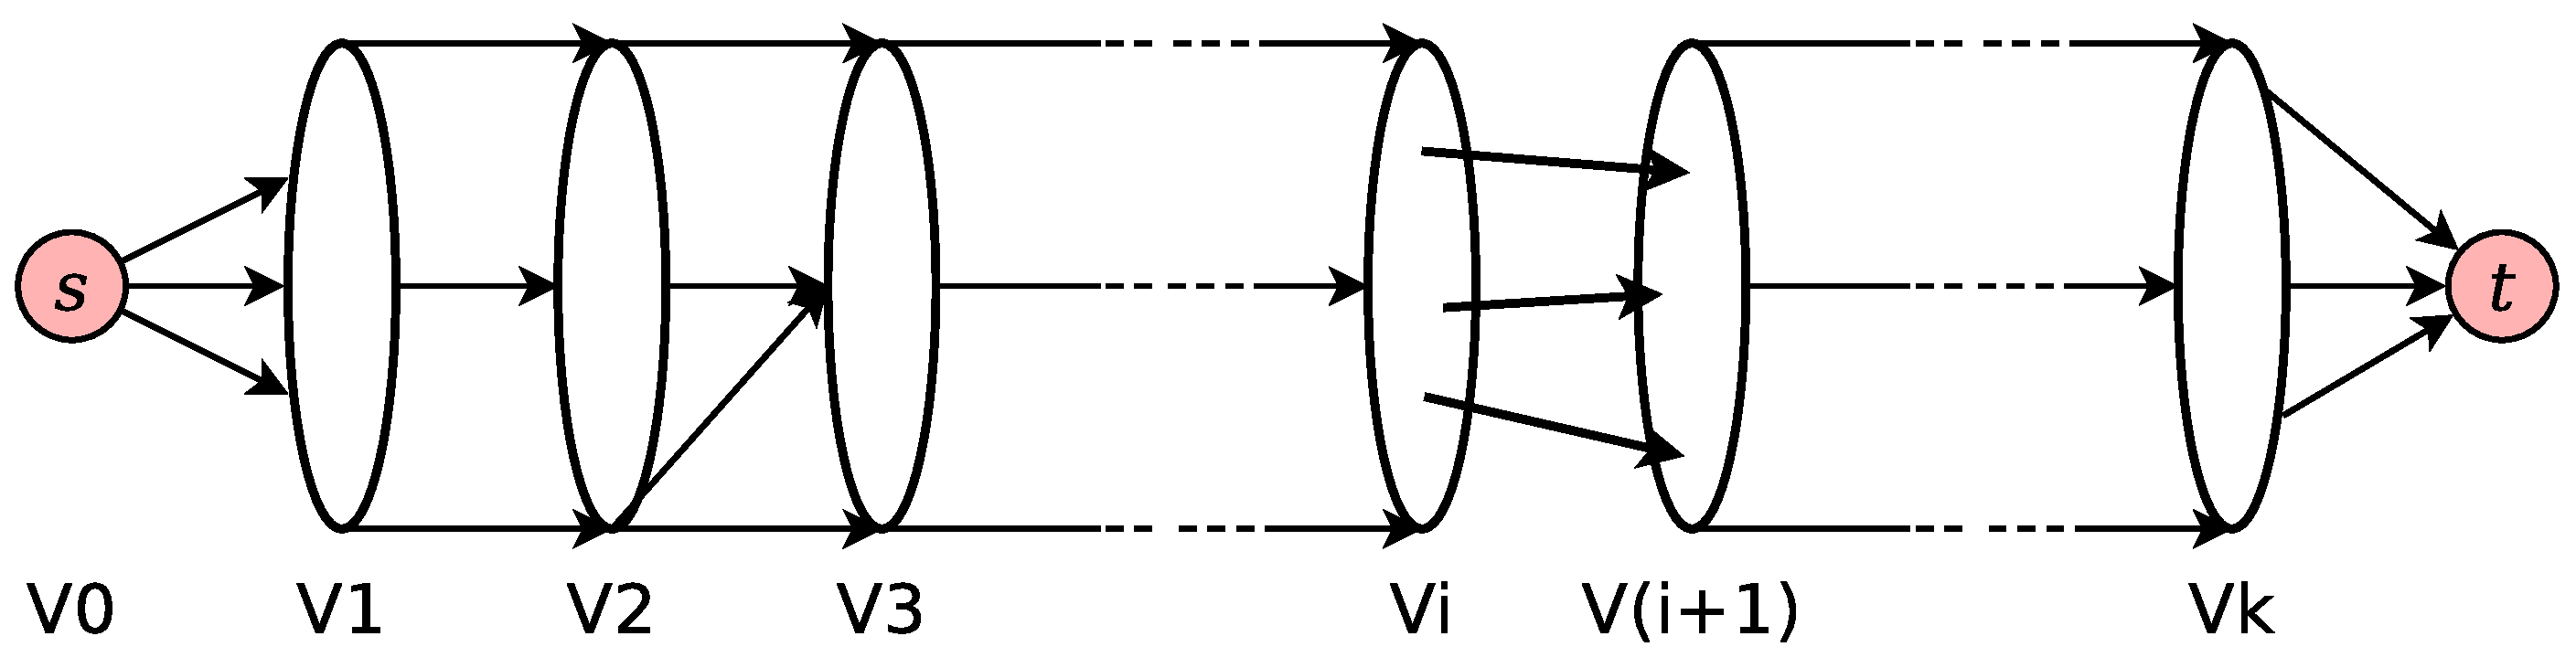
\includegraphics[width=\linewidth]{28/Grafik/Diagramm1}
\caption{Schaubild}
\label{fig:Diagramm1}
\end{figure}
\paragraph{Behauptung}
\begin{flushright}
	$k=2\cdot|V|^\frac{2}{3}$
\end{flushright}
\begin{align*}
 \exists 0<i<k:&|V_i|\leq |V|^\frac{1}{3}\\
 \text{und }&|V_{i+1}|\leq |V|^\frac{1}{3}
\end{align*}

Falls Behauptung gilt $\Rightarrow ~~c_f(V_i,V_{i+1}) \leq \#\text{Kanten über diesen Schnitt}\leq |V_i|\cdot|V_{i+1}| \leq|V|^\frac{2}{3}$. Maximaler Fluss $|f^*|$ ist vom aktuellen Fluss $f$, der sich nach der 1. Phase eingestellt hat höchstens noch $|V|^\frac{2}{3}$ entfernt. Deshalb genügen in der 2. Phase noch $|V|^\frac{2}{3}$ Sperrflussberechnungen um $|f^*|$ zu erreichen.
\pagebreak
\paragraph{Beweis der Behauptung}
$<|V|^\frac{2}{3}$ Schichten haben $>|V|^\frac{1}{3}$ Knoten. Andernfalls gäbe es mehr als $|V|^\frac{2}{3}\cdot|V|^\frac{1}{3}=|V|$ viele Knoten.
\subparagraph{Beweisidee}
Wir färben die Schichten weiß, welche weniger als $|V|^\frac{1}{3}$ Knoten haben und den Rest schwarz, da es mehr weiße als schwarze gibt, müssen 2 weiße aufeinander folgen.:
\[ \underset{k}{\underbrace{w~s~w~s~w~s~\ldots~w~s}} \]

$>|V|^\frac{2}{3}$ Schichten haben $\leq |V|^\frac{1}{3}$ Knoten\\
$\Rightarrow$ es muss $i$ geben, mit $|V_i|\cdot|V_{i+1}|\leq |V|^\frac{1}{3}$
\begin{flushright}
	q.e.d.
\end{flushright}
\subsection{Finden knotendisjunkter Wege}
\paragraph{Idee} Man Forme den Graphen wie folgt um:
\begin{figure}[H]
\centering
\begin{subfigure}[H]{0.4\linewidth}
	\centering
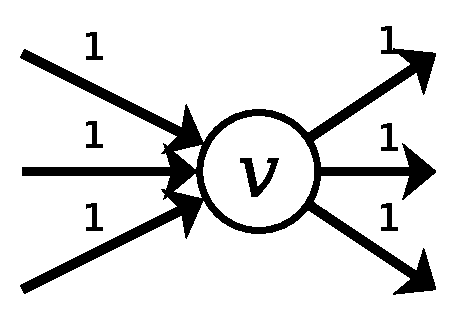
\includegraphics[width=0.5\linewidth]{28/Grafik/Diagramm2}
\caption{Original Knoten}
\label{fig:Diagramm2}
\end{subfigure}
\begin{subfigure}[H]{0.4\linewidth}
	\centering
	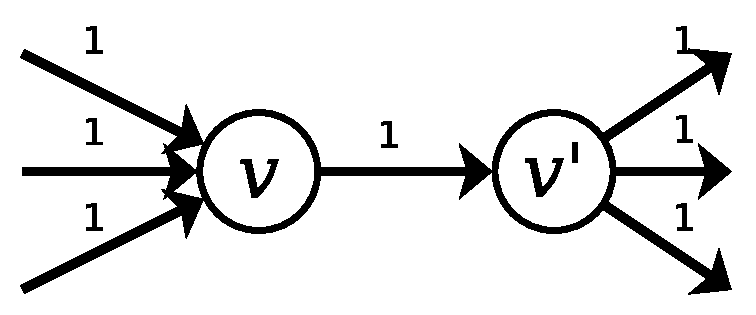
\includegraphics[width=\linewidth]{28/Grafik/Diagramm3}
	\caption{Umgeformter Knoten}
	\label{fig:Diagramm3}
\end{subfigure}
\end{figure}
\subsection[Ergänzung zum Paper]{Ergänzung zum Paper\footnote{\href{http://www.sciencedirect.com/science/article/pii/0020019078900169}{Information Processing Letters Volume 7, number 6}}}

\[ \pot_f(v)=\min\left( \sum_{(v,u)\in E}c(v,u)-f(v,u),\sum_{(u,v)\in E}c(u,v)-f(u,v) \right) \]
\begin{figure}[h]
\centering
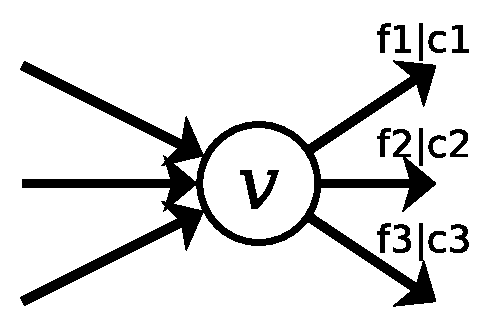
\includegraphics[width=0.2\linewidth]{28/Grafik/Diagramm4}
\caption{}
\label{fig:Diagramm4}
\end{figure}

